\chapter[Accommodation Module for Spoken Dialogue Systems]{Accommodation Module for\\Spoken Dialogue Systems}
\label{chap:convergence_module_for_sdss}

\lettrine{T}{his} chapter introduces a plug-and-use module for \acs{sds} that adds support for vocal accommodation.
It is integrated into the system as a new link between the \acs{asr} and \acs{tts} modules.
The implementation and integration details as well as a demonstration of manipulating the system's output using this module are presented and discussed.

\pagebreak

\section{Modularization}
\label{sec:modularization}

An implementation of the pipeline introduced in \cref{sec:pipeline_representation} is presented here as an independent module for \acp{sds}.
It is shown how the statistical components from \cref{chap:statistical_model} can be added to it to take advantage of the capabilities of both approaches.
This suggested implementation is an example of how the model works while keeping the complexity of each step to a minimum.
While supra-segmental features can be handled as well, only segmental features are discussed here, as they are less represented in accommodation modeling for computer-based systems and they require additional considerations, like segment context and local manipulation, as demonstrated in this chapter (and see \citet{Raveh2017SemDial}).
Thanks to the independence of this module, it can be added into any existing system that can provide the user's speech signal as input and a \ac{tts} module that can receive its output.
The \ac{sds} presented in \cref{chap:web-based_responsive_spoken_dialogue_system} has the \ac{asp} module integrated into it.

\subsection{Computational model}
\label{subsec:computational_model}

The implementations of the pipeline's steps will be explained using the following feature definition example, which describes the feature \emph{@\_length}, i.e., length of a segment containing the phoneme schwa (\textipa{[@]}, and cf.\ \cref{subsec:target_features_HCIConv}):
%
\begin{Verbatim}[tabsize=4, commandchars=\\\{\}]
	- \textbf{`@\_length'}:
			\textbf{phoneme}: AX
			\textbf{context}: '.+ AX N'
			\textbf{initial}: 0
			\textbf{minimum}: 0 
			\textbf{maximum}: 80
			\textbf{measure}: duration
			\textbf{calculation}: average
			\textbf{sensitivity}: 0.5
\end{Verbatim}
%
The entire implementation is described in \cref{alg:comp_model}.
Further details about the model and all the steps can be found in \citet{Raveh2017Interspeech}.

\subsubsection{Detecting segment exemplars}
\label{subsubsec:detecting segment exemplars}

The first step in the model's pipeline is detecting segments in the user's utterance that can be ascribed to target features defined for the system.
These features are defined in a configuration file that is loaded by the model.
For that, an \ac{asr} engine that emits phoneme times is required.
Here, CMU Sphinx\footnote{\url{https://cmusphinx.github.io/}} was used, with extended functionality to support the emission of phoneme-level information.
This additional functionality was built specifically for this purpose (and as part of the system described in \cref{chap:web-based_responsive_spoken_dialogue_system}), with an emphasis on phoneme-boundary accuracy.
Each feature is represented by a YAML\footnote{YAML Ain't Markup Language \url{http://yaml.org/}} dictionary entry, which in turn contains a dictionary itself, where each key-value pair refers to a property of that feature that is relevant for the system's accommodation.
Concretely, the phoneme \textipa{[@]} is labeled as \emph{AX} in the German CMU phonemeset, which was the phonemeset used in CMU Sphinx.
This is defined by the \texttt{phoneme} key in the feature definition above.
The key \texttt{measure} sets the measure by which this feature is evaluated; here, its duration.
Other measures are \enquote{formants} (for vowel quality), \enquote{category} (for categorical differences), and more.
This feature's initial value in the system's representation for it is set by the \texttt{initial} key.
This step is performed for each feature separately against each recognized phoneme (see \cref{alg:comp_model}).
Phonemes not ascribed to any defined feature are ignored.

\subsubsection{Filtering exemplars}
\label{subsubsec:filtering_exemplars}

Seeing that segmental features are detected merely based on a phoneme in which they \emph{may} occur, additional filtering is required to retain only those instances where they do.
For example, the target feature \emph{@\_length} introduced in \cref{subsubsec:detecting segment exemplars} aims to capture the German phonological process of elision or epenthesis of \textipa{@} in word-final \emph{<-en>}.
%
%(simplified version adapted from \citet[pp.\,142--143]{Benware1986phonetics}):
%
%\begin{equation}
%	\label{eq:schwa_elision_rule}
%	\text{\textipa{@}}\longrightarrow \varnothing \diagup
%	\left[\text{-son}\right] \ \_\_ \ \{\text{\#}, \left[\text{+const}\right]\}.
%	\todo{this rule is already defined in \cref{eq:}}
%\end{equation}
%\eqname{Phonological rule: schwa elision}
%
This filtering step comes to add any linguistic considerations related to the phonetic feature in question beside the phoneme itself.
Such considerations can be phonemic context, defined as a phoneme regular expression in the \texttt{context} property, a range of acceptable values, defined by the \texttt{minimum} and \texttt{maximum} keys, or both.
In the case of \emph{@\_length} feature above, only segments appearing in the phonemic context corresponds to a (simplified) context of the phonological rule described in \cref{eq:schwa_elision_rule} are considered, and the feature's representation cannot go above 80 (\si{\milli\second}).
The range's role is to filter out segments with unrealistic values (extremely long segment, unreliable formant values, etc.).
For example, a schwa segment longer than \SI{80}{\milli\second} would sound very unnatural.
Any linguistic knowledge about the feature nature can be reflected in this step.
This is important to make sure that all exemplars are taken into account when calculating a new value for the feature (see \cref{subsubsec:calculating_changed_value} are sensible, to prevent unstable behavior of the model due to lack of linguistic knowledge or \ac{asr} errors.

\subsubsection{Storing exemplars}
\label{subsubsec:collecting_exemplars}

The remaining exemplars are stored and can be represented by a matrix, which contains the values of these exemplars.
Since each feature is tracked separately, each matrix $\mathcal{F}$ contains exemplars of a single feature, where each exemplar is a row and each column is a dimension of this feature (e.g., a formant in a vowel quality feature).
For instance, the matrix in
%
\begin{equation}
	\label{eq:feature_matrix}
	\mathcal{F}_{exemplar-view} =
	\begin{bmatrix} 
		v_{11} & v_{12} & \dots  & v_{1m}\\
		v_{21} & v_{22} & \dots  & v_{2m}\\
		\vdots & \vdots & \ddots & \vdots\\
		v_{n1} & v_{n2} & \dots  & v_{nm} 
	\end{bmatrix},
\end{equation}
\eqname{A matrix of a phonetic feature}
\noindent
%
the value $v_{21}$ is the first dimension of the second exemplar of the feature.
The model also defines a \emph{pool size}, which determines how many exemplars are kept for each feature.
This parameter aims to represent short-term mental memory of a feature's pronunciation.
When a new exemplar is stored, it is added to the pool (a memory matrix).
When a feature's pool is reached its maximal size, the oldest exemplar is removed (forgotten) to make space for the newest one.
The exemplars in the pool are later used for calculating the system's change (\cref{subsubsec:calculating_changed_value}).
To calculate the change for each dimension, the feature matrix is first transposed, as in
%
\begin{equation}
	\label{eq:transposed_feature_matrix}
	\textbf{$\mathcal{F}_{dimension-view}$} =
	\begin{bmatrix} 
		v_{11} & v_{21} & \dots  & v_{n1}\\
		v_{12} & v_{22} & \dots  & v_{n2} \\
		\vdots & \vdots & \ddots & \vdots \\
		v_{1m} & v_{2m} & \dots  & v_{nm} 
	\end{bmatrix},
\end{equation}
\noindent
%
where each row refers to a single \emph{dimension} of the feature, rather than an exemplar.

\subsubsection{Calculating a new value}
\label{subsubsec:calculating_changed_value}

The new value of a feature is calculated based on its exemplar pool.
The way the values in the pool are used to determine the change in the system's representation of the feature is a key aspect of the accommodation process.
A \emph{calculation method} is needed to define this relationship.
Different calculation methods can represent different types of relations and approaches.
For example, it can be simulated that people are more likely to converge to utterances they heard recently than to something they heard before.
A function $g$ is defined so that it maps a vector to a scalar (i.e., one feature dimension) and a function $\mathcal{G}$ which maps a matrix to a vector (the entire feature) by applying $g$ to all the row vectors in $\mathcal{F}$:
%
\begin{equation}
	\label{eq:matrix2vec}
	\mathcal{G}: \mathbb{Q}^{n \times m} \longrightarrow \mathbb{Q}^{m}, \qquad g: \mathbb{Q}^{m} \longrightarrow \mathbb{Q}.
\end{equation}
%
\noindent
Importantly, any function that maps vectors to scalars can be used to experiment with different methods.
For the demonstration in \cref{sec:showcase} decaying average is used (see \cref{subsubsec:tracked_features} for details).

Before setting the updated value as the feature's value, the balance between the feature's current value and its calculated pool value needs to be set.
This is defined by the \texttt{sensitivity} (convergence rate), which determines the sensitivity of this feature (see \cref{sec:parameters}) and is implemented as
%
\begin{equation}
	\Upsilon \equiv \mathcal{C}_u = \rho \upsilon + \left(1 - \rho \right) \mathcal{C}_{u-1},
	\label{eq:convergence_rate}
\end{equation}
\eqname{Sensitivity (convergence rate)}
\noindent
%
where $\Upsilon$ is the new feature value, $\upsilon$ is the calculated pool after applying $\mathcal{G}$, $\mathcal{C}_{u-1}$ is the current value of the feature, and $\rho$ is the convergence rate.
A $\rho$ value of 0 means that no convergence occurs (the current value is retained), a value of 1 will result in complete convergence (the current value is ignored), and $\rho=0.5$ will result in an average between the two.
While the convergence rate is typically a value between 0 and 1, smaller and greater values could be meaningful in some applications to achieve over-divergence or over-convergence, respectively.
As shown in \cref{part:experiments}, peoples' accommodation may vary considerably in \acp{hhi} and \acp{hci} and different settings.
This parameter can help to tune the system's behavior to achieve the desired behavior in the interaction.
For instance, in a tutoring system for pronunciation training, the desired behavior might be for the system to diverge from users' input when it detects that their pronunciation is wrong.
By reflecting the users' utterance with diverged pronunciation (instead of explicitly pointing out their mistake), the user receives auditory feedback in a more implicit, \enquote{conversational} learning process.

%\begin{equation}
%	\lambda\mathcal{M} = \lambda
%	\begin{pmatrix} 
%		v_{11} & v_{12} & \dots  & v_{n}\\
%		v_{21} & v_{22} & \dots  & v_{2n} \\
%		\vdots & \vdots & \ddots & \vdots \\
%		v_{e1} & v_{e2} & \dots  & v_{en} 
%	\end{pmatrix}
%\end{equation}
%
%\begin{equation}
%	\mathcal{M}_i' = g(\mathcal{M}^{\intercal}_{i \leq m})
%	\label{eq:value_calculation}
%\end{equation}
%\noindent
%where $\mathcal{M}^{\intercal} \in \mathbb{Q}^{m \times n}$ is the transposed exemplar matrix (which comprises vectors of dimension values instead of vectors of exemplar values), $g$ is the chosen calculation method to apply to each vector, $\mathcal{M}' \in \mathbb{Q}^{m \times n}$ is the matrix with the pool values for each dimension of the feature, $i$ is the vector index, and $m$ is the number of rows in $\mathcal{M}^{\intercal}$.

%$\lVert P \rVert $ refers to the Euclidean Norm (or vector's magnitude).

\subsubsection{Setting the new value}
\label{subsubsec:setting_the_new_value}

The final step is to set the newly calculated value as the new value for the feature in the system's representation.
After this step, this new value will be used whenever this feature is used by a system using this model (as shown in \cref{subsec:extended_sds}).
Although this step is fairly straight forward, there is still an important issue to take into consideration here, namely \emph{user imitation}.
After some turns, it might happen that the model calculated a value very close to the user's input and then continues to follow the user's production values, resulting in imitation of the user.
To avoid imitation, the new value is limited in how close it is allowed to get to the exemplars.
This is done by the global property \emph{ConvergenceThreshold}, which defines the maximally allowed proximity (in percentage) the new value is allowed to have:
Setting this property to 0.8 (\SI{80}{\percent} means that the new value is not allowed to be changed more than (\SI{80}{\percent} of the difference between the current value and the pool's value (and be set to (\SI{80}{\percent} in case it exceeded this threshold).
Of course, the limitation can also be set to 1 to allow the new value to be as similar as \SI{100}{\percent} to the pool's value -- i.e., not limiting it.
The maximal value allowed by the limitation is defined by
%
\begin{equation}
	\label{eq:conv_limit}
	\Lambda = \delta \upsilon \left(1 - \lambda \right),
\end{equation}
\noindent
%
where $\Lambda$ is the maximum convergence value allowed, $\delta$ is set to 1 if the converging values are increasing or $-1$ in case they are decreasing (see \cref{eq:direction}), and $\lambda$ is the convergence limit parameter ($\lambda=0.8$ in the example above).
\noindent
Note that the actual value of this limit depends on the direction in which the convergence occurs, which is defined by
%
\begin{equation}
	\label{eq:direction}
	\delta = 		
	\begin{cases}
		\ \ \ 1 & \text{if } \upsilon \geq \mathcal{C}_t\\
		-1 & \text{otherwise}
	\end{cases}.
\end{equation}
\eqname{Determining accommodation direction}
\noindent
%
That is, if the converging values are increasing, the limit's value will be smaller than the pool value;
and if the values are decreasing toward the pool value, the limit's value will be greater than the pool value.
Ultimately, the final updated value for the feature is determined as follows:
%
\begin{equation}
	\label{eq:new_value}
	\Upsilon = 		
	\begin{cases}
		% newValue - (newValue - (newValue * convergenceThreshold)) * direction
		\upsilon - \Lambda & \text{if }\upsilon - \Upsilon \leq \delta\Lambda\\
		\Upsilon \text{ (unchanged)} & \text{otherwise}
	\end{cases}.
\end{equation}
\eqname{Setting accommodation limit}
\noindent
%
It is important to mention that this limitation not only comes to prevent situations where the model imitates the user's behavior but is also loyal to empirically observed behaviors in \cref{chap:shadowing_experiment_with_natural_and_synthetic_voices,chap:speech_variations_in_hhci}, where participants typically converged only up to a certain limit.

\addtocounter{myequations}{1}
\begin{algorithm}[h!]
	\caption{Phonetic responsiveness}
	\label{alg:comp_model}
	\eqname{Phonetic responsiveness algorithm}
	\algorithmcaption{Note that \emph{ASRInput} (\cref{line:asrinput}) must not only contain the $n$-best hypotheses, but also their phoneme lists (in chronological order).
	For improving performance, using a single hypothesis is recommended for a small language model and/or when very short sentences are expected.
	Since only the target phonemes are treated (and suprasegmental features where the specific phonemes do not matter), it might not be crucial to get a completely correct \ac{asr} hypothesis if not required for continuing the interaction.
	For example, a \ac{capt} system might rely solely on the realization of specific phonemes, regardless of what the user said or should have said.}
	\DontPrintSemicolon
	\SetKwInOut{Input}{Inputs}
	\SetKwInOut{Output}{Output}
	
	\Input{\underline{$ASRInput$} -- phonemes from recognized user speech\newline
		   \underline{$targetPhonemes$} -- convergence features\newline}
	\Output{feature vectors with accommodated values\newline}
	
	\ForEach {(phoneme $\in$ ASRInput) $\in$ targetPhonemes}{ \label{line:asrinput}
		$feature \gets$ $phoneme$.associatedFeature\;
		$context \gets feature$.phoneticContext\;
		\;
		\uIf(\tcp*[f]{filter based on context}){\textbf{not} matches(phoneme, context)}{
			break\;}
		\;
		\uIf(\tcp*[f]{filter based on range}){inRange($phoneme$, $feature.allowedRange$)}{
			\uIf {poolSize=maxPoolSize}{
				deleteOldestExemplar()\;}
			feature.addExemplar($phoneme$)\;}
		\uElse{
			break\;}
		\;
		\uIf {toUpdate $=0$}{
			$method \gets feature$.calculationMethod\;
			$poolValue \gets method$.calculate(pool)\;
			$newValue \gets rate\cdot poolValue + (1-rate)\cdot feature.$currentValue\;
			$threshold \gets convergenceLimit \cdot poolValue$\;
			\;
			\uIf(\tcp*[f]{limit convergence}){$newValue > threshold$}{
				$newValue \gets threshold$\;}
			$feature$.value $\gets newValue$\;
			{\em toUpdate $\gets$ updatefrequency}\;}
		\uElse{
			{\em toUpdate $\gets$ toUpdate - 1}\;}}
\end{algorithm}

\subsection{Statistical model}
\label{subsec:statistical_model}

While the computational model covers all the required steps for processing changes, its division into independent steps makes it possible to replace specific steps with alternatives.
Specifically, the \emph{update} step, which is responsible for the actual change in the feature's representation, can use different techniques for doing so.
The input for this step is a history of exemplars (the pool) and its output is a new value for the feature.
These are exactly the input and output of the statistical model introduced in \cref{chap:statistical_model}.
Therefore, it may be substitute this step to generate variational accommodative behavior, if needed.
One of the potential issues in the statistical model is choosing the input values for the generation.
This is especially challenging when dealing with segmental features, which might not occur as regularly as supra-segmental features, and thus make the filtering trickier.
As part of the pipeline, the \emph{store} step takes care of collecting the relevant exemplars and decide how to treat each of them when calculating the next value.
Combining the computational and statistical models lets the system enjoy the benefits of both and give the system designer more degrees of freedom when creating different applications.

\section{Integration}
\label{sec:integration}

\subsection{Extended \acl{sds} architecture}
\label{subsec:extended_sds}

The accommodation process can now be utilized, using the implementation described in \Cref{sec:modularization}, and it can now be integrated into a \ac{sds} with a standard architecture (cf.\ \Cref{fig:sds_architecture}) as a separate module.
As this module relies on input from the \ac{asr} module and its output is consumed by the \ac{tts} module, it is inserted as a new, direct link between the two, in addition to their connections to the \ac{nlu} and from the \ac{nlg} modules, respectively.
\Cref{fig:adaptation_module_architecture} shows these connections.
The name of this module, \acf{asp}, does not refer to accommodation, as it could, in principle, be used for other purposes as well.
This may include any processing relying on the user's speech signal, besides transcription.
Since the speech signal is discarded after the \ac{asr} module finishes its processing, not speech-related analysis can be sent as input to the other modules.
Here, this is leveraged by the \ac{tts} module, but such analyses could be useful for also for the \ac{dm} or \ac{nlg} modules, e.g., for matching the response content to the user's mood based on voice characteristics \citep{Braun2016assessing, Rothkrantz2004voice}.
%
\begin{figure}[t]
	\centering
	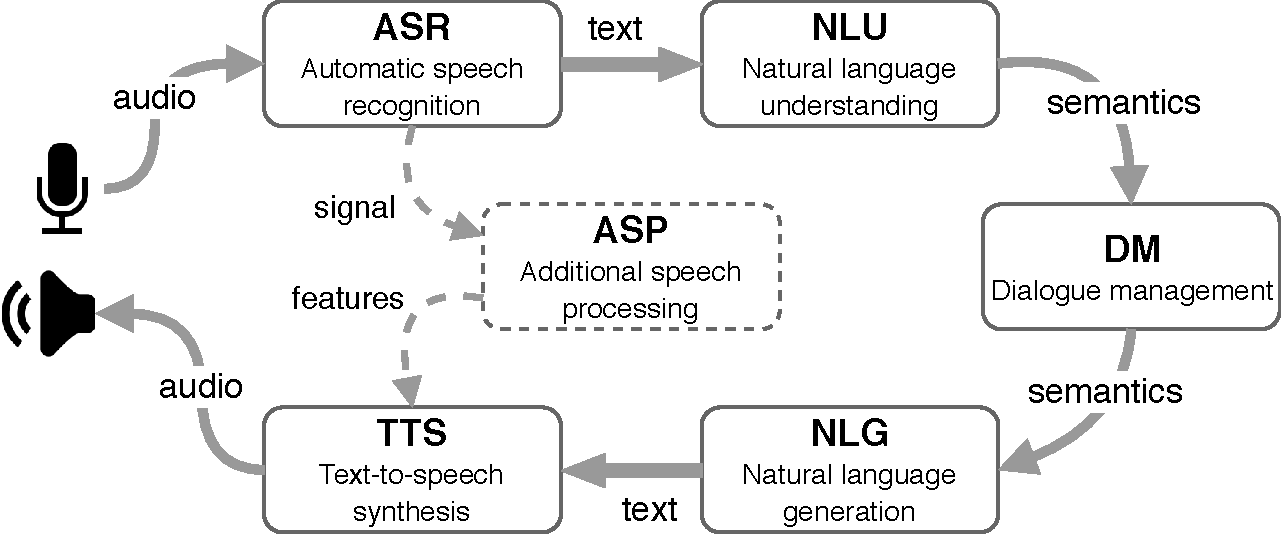
\includegraphics[width=\linewidth]{sds_architecture_ext}
	\caption[Proposed extended architecture of a spoken dialogue system]
		{Suggested architecture for a spoken dialogue system with the phonetic convergence module (cf.\ \cref{fig:sds_architecture}).
		The \acs{asp} module adds a direct link between the \ac{asr} and the \ac{tts} modules to perform additional speech processing used for phonetic accommodation.}
	\label{fig:adaptation_module_architecture}
\end{figure}

\subsection{Speech manipulation}
\label{subsec:speech_manipulation}

Although, as explained in \cref{subsec:extended_sds}, the \ac{asp} module is not responsible for the synthesis of the system's speech output, it is important to show that the information it provides could indeed be relevant for speech synthesis.
This is especially important, as the synthesis, along with the required changes for expressing accommodation, need to be applied \emph{in real-time} and cannot be learned offline from the input.
The examples given here focus on segmental features, because real-time manipulation techniques for  them are less common than for supra-segmental features like \ac{f0} and \ac{ar}.
\todo{need reference for this?}
For segmental features, modifications are applied to specific sounds occurring within short timespans, as oppose to supra-segmental features where longer segments (or the entire utterance) are influenced.
The challenge is, therefore, to apply these modifications without distorting the surrounding segments, to maintain the overall smoothness of the synthesized speech.
First, it is required to obtain the timespans to manipulate.
These can be usually provided by the \ac{asr} component of the system (see \cref{subsubsec:detecting segment exemplars}).
Then, the manipulation itself takes place.
What aspect of the signal is modified depends on the target feature.
For instance, the first two formants of an allophone's categorical variant are targeted in the examples below.
Finally, the manipulated segment needs to be connected to the rest of the segment while minimizing the distortion.
The way the latter two steps are executed depends on the technique used for the manipulation.
This is demonstrated here by two examples:
One for the \emph{\textipa{[e]} vs.\ \textipa{[E]}} feature, using an approach based on the source-filter theory \citep{Fant1970acoustic}; and one for the \emph{\textipa{[\c{c}]} vs.\ \textipa{[k]}} feature, using a neural approach (both features are described in \cref{subsec:target_features_HCIConv}).
Note that the former feature varies on a continuum (the formant space), while the latter is a discrete change between two categories (a fricative or a plosive).
The main difference between the two approaches is when the manipulation is done.
In the former, the modifications are post-synthesis on an existing audio signal, while in the latter the desired modifications are sent to the synthesizer's as part of its input and can be directly taken into account.
The advantage of this approach is that the resulted signal is more likely to be smoother, as it is not changed after created.
However, the neural approach is prone to overall lesser quality if it is not adequately trained to support changes to the target features.
This would influence not only the timespan of the manipulated feature, but the entire generated signal.
Additionally, such \ac{e2e} methods also lack the freedom of directly controlling the manipulation, which may be crucial for achieving the desired final output.
Moreover, for research and evaluation purposes, it is convenient to have both the original and modified signals for comparison and be able to directly control how the changes are applied.
%
%\begin{landscape}
%	\begin{figure}[t]
%		\centering
%		\hspace*{-2cm}
%		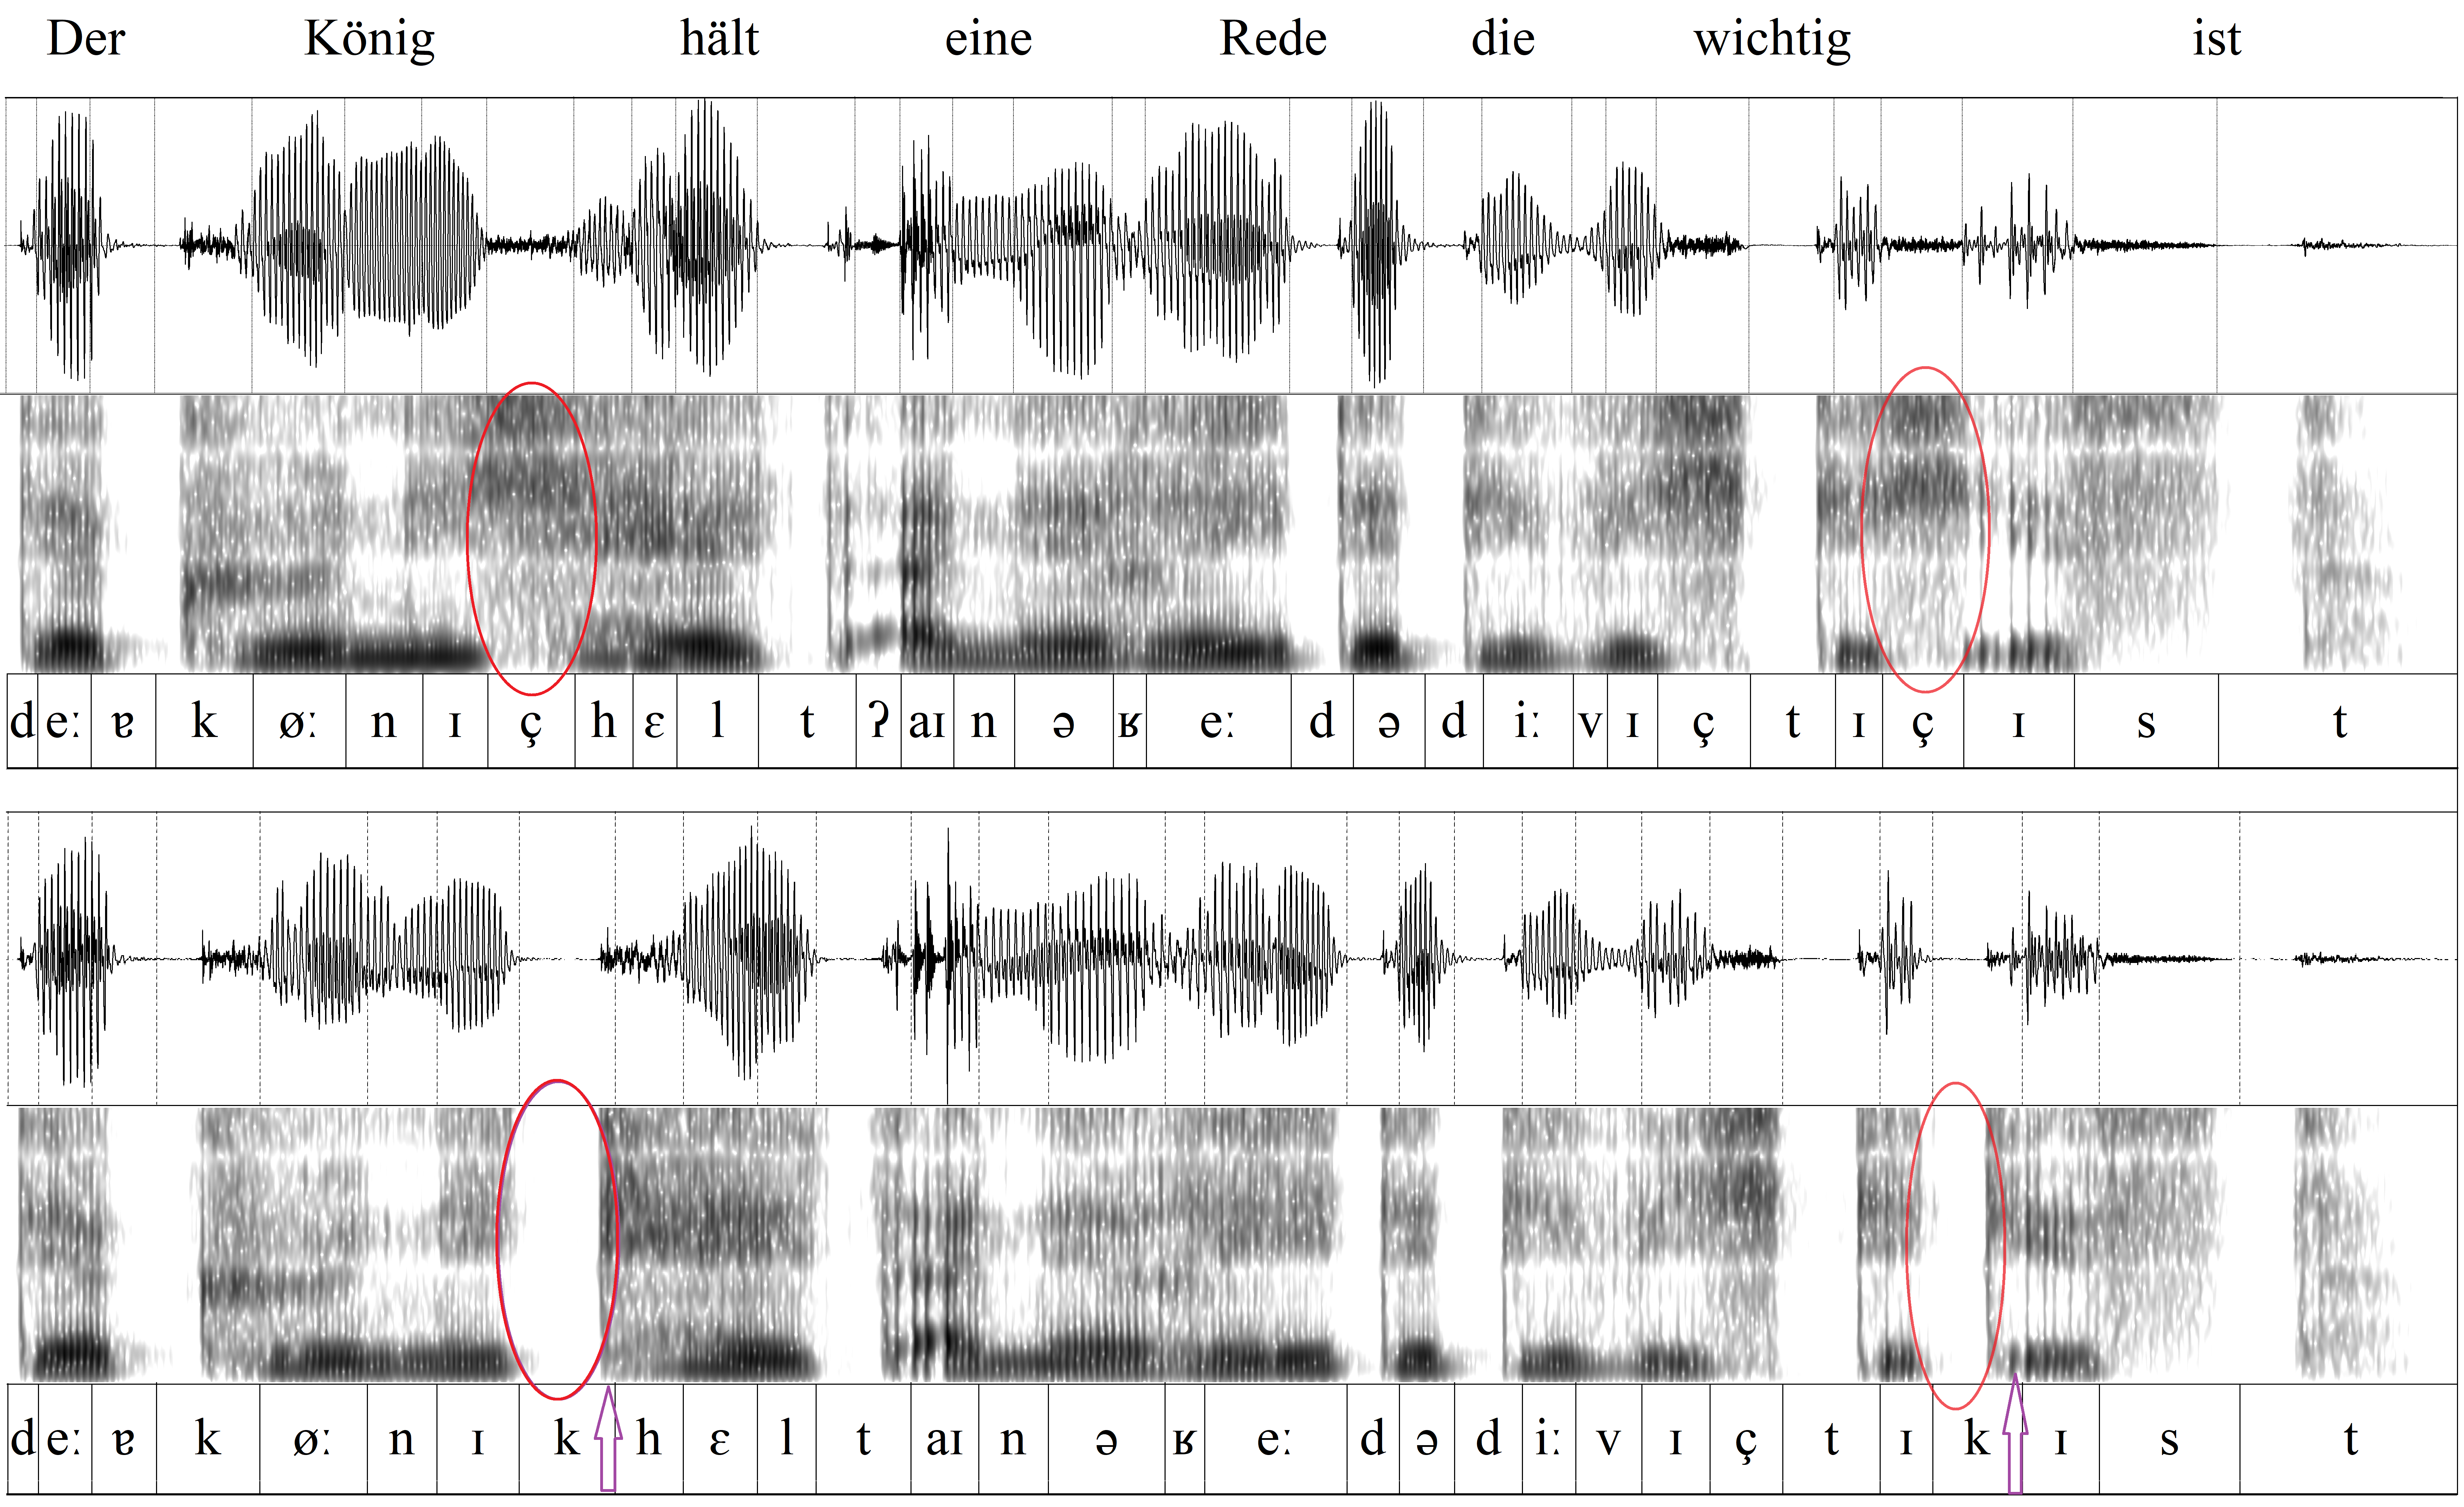
\includegraphics[width=1.5\textwidth]{ic_ik_manipulation}
%		\caption[]
%			{}
%		\label{fig:spectrogram_e_E}
%	\end{figure}
%\end{landscape}
%

%\missingfigure{spectrogram comparison for e/E feature}

The source-filter manipulation was done as follows:
First, the formant contours were extracted from the audio signal.
this was done by computing the LPC coefficients with the algorithm by Burg, as given by \citet{Press1989numerical}.
One value was extracted per formant every \SI{6}{\milli\second}.
% with linear interpolation for missing values.
Then, the first and second formants of the vowel target were changed separately.
The changes were based on the respective means of the formants in the duration of the target vowel, while taking the overall contour into account.
Finally, The original signal was used as the source and was filtered by the manipulated formant contours, resulting in a new speech signal that differs from the original only by the target vowel's segment.
% for the first method, it is also necessary to re-synthesize the audio (overlap-add Moulines & Charpentier (1990), who called it Time-Domain Pitch-Synchronous Overlap-and-Add (TD-PSOLA))
The neural-based manipulation is based on Tacotron\footnote{Tacotron2 architecture based on the implementation in the repository \url{https://github.com/NVIDIA/tacotron2}} \citep{Shen2018natural}, which is trained to generate spectral information directly from textual input.
To capture the categorical phoneme variance of the feature \emph{\textipa{[\c{c}]} vs.\ \textipa{[k]}}, the system was trained on \emph{phoneme} input (as opposed to orthographic forms).
For this, the neutral voice subset of the PAVOQUE dataset\footnote{\url{https://github.com/marytts/pavoque-data}} \citep{Steiner2013pavoque} was used, which comprises $\sim$\SI{5.8}{\hour} of speech.
The phonetic transcriptions were done automatically based on the transcriptions provided with the dataset and were manually verified and corrected.
\todo{need more details?}
After training, the model was able to generate synthesized speech based on an input of an arbitrary phoneme sequence.
This opens many possibilities, one of them is alternating between \textipa{[\c{c}]} and \textipa{[k]} to express the variation of this feature.
It is important to note that the other-category variant of a word was not included in any dictionary and was not seen by the model during training.
\Cref{fig:spectrogram_ic_ik} shows an example of an original sentence (pronounced with \textipa{[\c{c}]} sounds) and its manipulated form (with \textipa{[k]} sounds).
%
\begin{landscape}
	\begin{figure}[t]
		\centering
		\vspace*{-2cm}
		\hspace*{-2cm}
		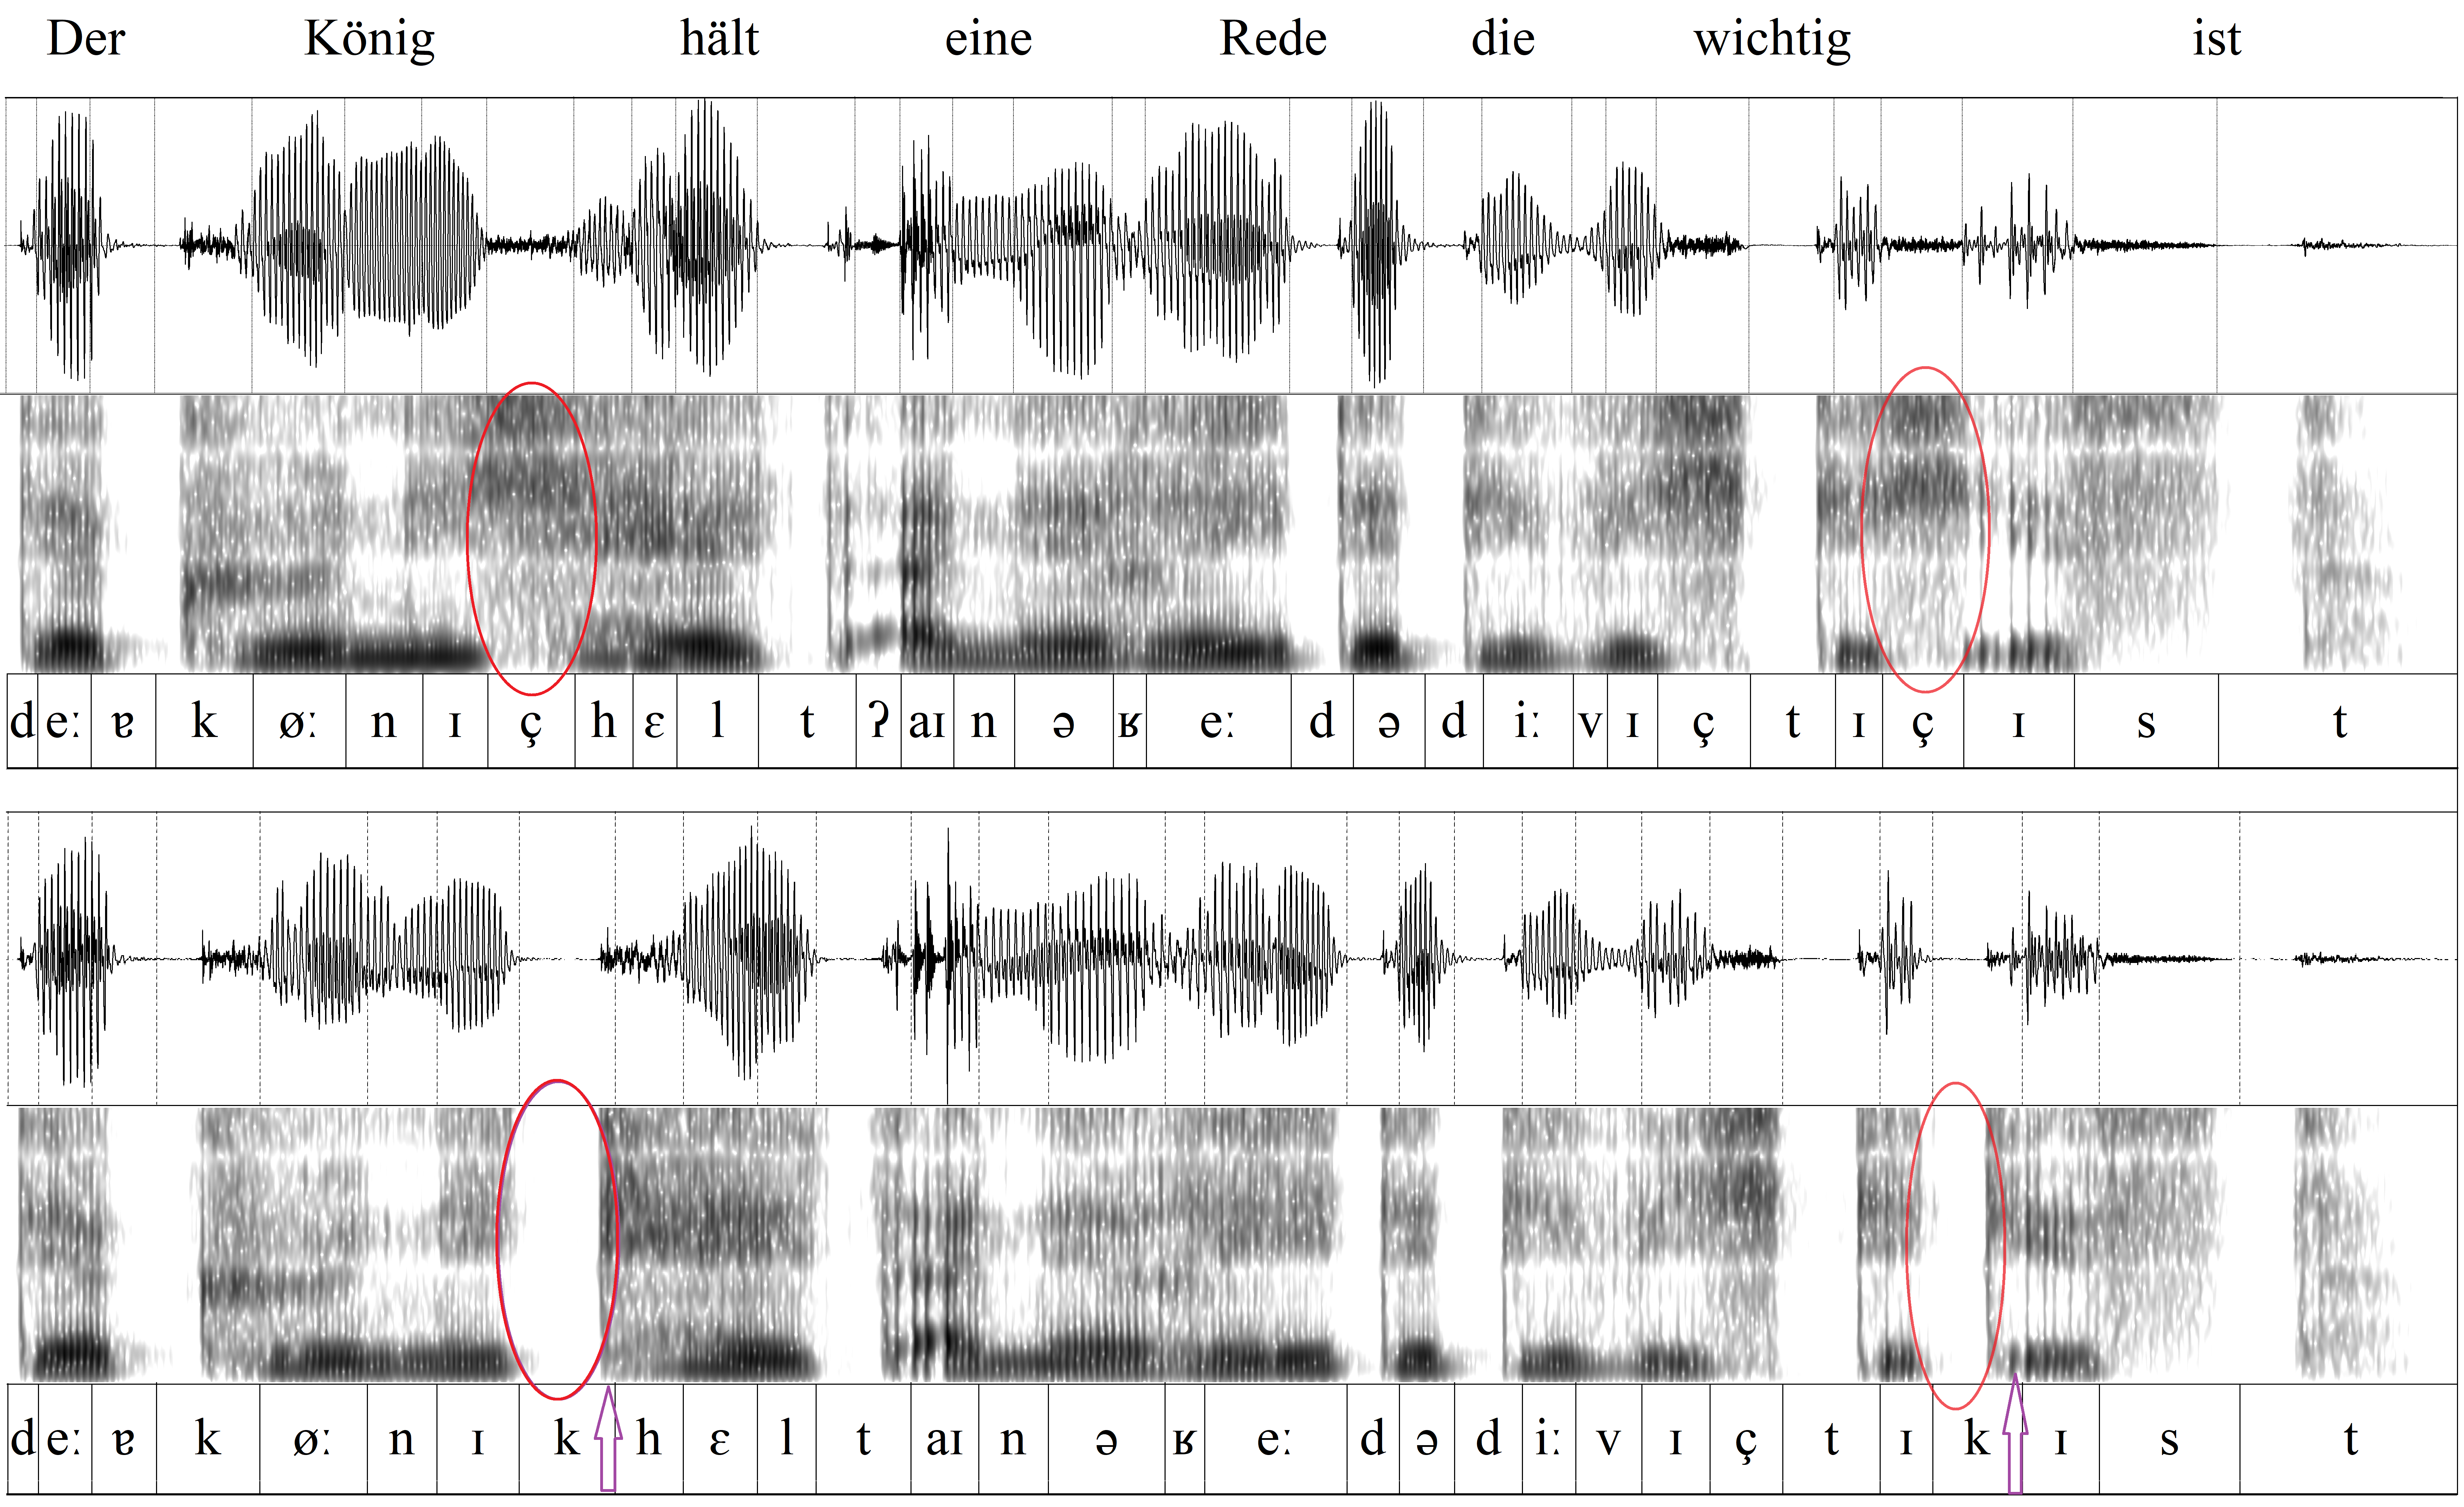
\includegraphics[width=1.5\textwidth]{ic_ik_manipulation}
		\caption[Oscillograms and spectrograms of categorical manipulation comparison]
			{Oscillograms and spectrograms of the word \emph{\enquote{König}} (king) and \emph{\enquote{wichtig}} (important) pronounced originally with \textipa{[\c{c}]} sounds, which were changed into \textipa{[k]} sounds.
			The x-axis shows the chronological phonetic transcription over time (\SI{2.34}{\second} in total) and the spectrograms' y-axes show the frequencies up to \SI{5000}{\hertz}.
			The segments of the modified phonemes are marked with red circles.
			The purple arrows at the end of the \textipa{[k]} segments show that the model even captured the voicing assimilation to the following vowel.
			The vertical lines show the phoneme segmentation.
			Note that the segments are not perfectly aligned in the two productions.}
		\label{fig:spectrogram_ic_ik}
	\end{figure}
\end{landscape}